\documentclass[a4paper,11pt]{article}

\usepackage[english]{babel} 
\usepackage[utf8]{inputenc}
\usepackage[cyr]{aeguill}
\usepackage{stmaryrd}

\usepackage{lmodern} %Type1-font for non-english texts and characters
\usepackage{caption}
\usepackage{subcaption}

\usepackage{graphicx}
\usepackage{hyperref}
\usepackage{listings}

\usepackage{epstopdf}

%% Math Packages 
\usepackage{amsmath}
\usepackage{amsthm}
\usepackage{amsfonts}
\usepackage{amssymb}
\usepackage{mathrsfs}
\usepackage{pst-all}
\usepackage{lscape}
\usepackage{pdfpages}
\usepackage{mathabx}


\usepackage{color, colortbl}
\definecolor{lightgray}{gray}{0.85}
\usepackage{multirow}
\usepackage[Algorithme]{algorithm}
\usepackage[noend]{algpseudocode}
\usepackage{tikz}

%\renewcommand{\algorithmicdo}{\textbf{faire}}
%\renewcommand{\algorithmicwhile}{\textbf{tant que}}


\usepackage{a4wide} %%Smaller margins = more text per page.
\usepackage{fancyhdr} %%Fancy headings

\setcounter{secnumdepth}{5}
\setcounter{tocdepth}{5}


\DeclareMathOperator*{\argmax}{arg\,max}
\DeclareMathOperator*{\argmin}{arg\,min}
\graphicspath{{/Users/melisandezonta/Documents/Documents/Documents/GTL_courses_second_semester/Computer-Vision/PS6-all/PS6-input/}}




\usepackage{listings}
\usepackage{color}
 
\definecolor{codegreen}{rgb}{0,0.6,0}
\definecolor{codegray}{rgb}{0.5,0.5,0.5}
\definecolor{codepurple}{rgb}{0.58,0,0.82}
\definecolor{backcolour}{rgb}{0.95,0.95,0.92}
 
\lstdefinestyle{mystyle}{
    backgroundcolor=\color{backcolour},   
    commentstyle=\color{codegreen},
    keywordstyle=\color{magenta},
    numberstyle=\tiny\color{codegray},
    stringstyle=\color{codepurple},
    basicstyle=\footnotesize,
    breakatwhitespace=false,         
    breaklines=true,                 
    captionpos=b,                    
    keepspaces=true,                 
    numbers=left,                    
    numbersep=5pt,                  
    showspaces=false,                
    showstringspaces=false,
    showtabs=false,                  
    tabsize=2
}
 
\lstset{style=mystyle}

\begin{document}

%\pagestyle{fancy}

\begin{titlepage}
\vspace*{\stretch{1}}

\begin{center}
\includegraphics[scale=0.4]{GT_logo.jpeg}
\end{center}
\vspace*{\stretch{1}}
\hrulefill
\begin{center}\bfseries\huge
   Computer Vision \\
   CS 6476 , Spring 2018\\
   \end{center}
  \begin{center}\bfseries\large
     PS 6\\
    \hrulefill
\end{center}
%\hfill
\vspace*{1cm}
\begin{minipage}[t]{0.6\textwidth}
  \begin{flushleft} \large
    \emph{Professor : }\\
    Cedric Pradalier \\
  \end{flushleft}
\end{minipage}
\begin{minipage}[t]{0.3\textwidth}
  \begin{flushright} \large
    \emph{Author :} \\
    Melisande Zonta \\
  \end{flushright}
\end{minipage}
\vspace*{\stretch{2}}
\begin{flushright}
       \today 
\end{flushright} 
\end{titlepage}

\tableofcontents
\clearpage

\section{Particle Filter Tracking}

\subsection{First Tracking}

After implementing the particle filter (see below), we use it to track Mitt Romney's face on the presidential debate video after extracting the template based on the accompanying text file (Figure 2).\\
We decided to use the standard deviation mentioned in the text for the MSE, and to add the same amount of noise to both the x and y position of the center.\\
The same value is used at the initialization and in the dynamics model, since it seemed to work best that way.
Moreover, since the movement of the face starts quickly in the video, having some initial spreading of the particles appears useful.
We get a pretty good result even after he turns his face (Figure 1). Although the patches content then does not match exactly the template, the appearance of his profile is not too far away, which explains the proper working of the tracker in this case.


\begin{table}[H]
\centering
\caption{Parameters}
%\label{my-label}
\begin{tabular}{|l|l|}
\hline
MSE standard deviation           & 10.0           \\ \hline
Initial noise standard deviation & {[}5. 5. 0.{]} \\ \hline
Predict noise standard deviation & {[}5. 5. 0.{]} \\ \hline
Number of particles              & 100            \\ \hline
\end{tabular}
\end{table}

\lstset{style=mystyle}
\lstinputlisting[language=Python, firstline=24, lastline=90]{/Users/melisandezonta/Documents/Documents/Documents/GTL_courses_second_semester/Computer-Vision/PS6-all/PS6-code/Functions.py}


\begin{figure}[H]
\begin{center}
\begin{tabular}{c}
	\includegraphics[height=1 \textwidth]{ps6-1-1-frames-28-84-144.png}\\
\end{tabular}
\end{center}
\caption{ps6-1-1-frames-28-84-144.png}
\label{ps-6-1-a}
\end{figure}

\begin{figure}[H]
\begin{center}
\begin{tabular}{c}
	\includegraphics[height=.2 \textwidth]{ps6-1-1-template.png}\\
\end{tabular}
\end{center}
\caption{ps6-1-1-template.png}
\label{ps-6-1-b}
\end{figure}

\subsection{Window Size Discussion}

In this section, we tried to increase and to decrease window size to see the impact on the tracker's accuracy.

\begin{table}[H]
\centering
\caption{Parameters}
%\label{my-label}
\begin{tabular}{|l|l|}
\hline
MSE standard deviation           & 10.0           \\ \hline
Initial noise standard deviation & {[}5. 5. 0.{]} \\ \hline
Predict noise standard deviation & {[}5. 5. 0.{]} \\ \hline
Number of particles              & 100            \\ \hline
Small scale                          &  0.1.           \\ \hline
Large scale                          &  2.5.          \\ \hline

\end{tabular}
\end{table}


We see in Figure 3 which used a large template (Figure 5) that increasing the 4
size of the template in this case does not have any real impact and our tracking is still good.
However, greatly reducing the size of the template (Figure 6), down to a tenth of its original size, our tracker gets lost and ultimately considers one of the stars in the background as a very likely candidate (Figure 4).
All in all, we could list some advantages of both approaches. Using one or the other will greatly depend on the specifics of the video and the target we wish to track.
\begin{itemize}
\item Small window: 
\begin{itemize}
	\item useful if the target contains a small detail that is constantly visible
and stands out from the rest of the video (e.g. eyes, QR code, etc) ; 
	\item possibly problematic if the target is moving fast, since the small size
of the window would make it easier to loose. 
\end{itemize}
\item Large window:
\begin{itemize}
        \item interesting since it takes a larger portion of the image and might be more robust for example when tracking an object that is rotating and standing out from the background ;
	\item pointless if the large window includes a sizable portion of the background and if this one is changing quickly (e.g. a pedestrian walking sideways in front of a succession of varying facades).
\end{itemize}
\end{itemize}

\begin{figure}[H]
\begin{center}
\begin{tabular}{c}
	\includegraphics[height=1 \textwidth]{ps6-1-2-frames-large-28-84-144.png}\\
\end{tabular}
\end{center}
\caption{ps6-1-2-frames-large-28-84-144.png}
\label{ps-6-2-a}
\end{figure}


\begin{figure}[H]
\begin{center}
\begin{tabular}{c}
	\includegraphics[height=.2 \textwidth]{ps6-1-2-template-large.png}\\
\end{tabular}
\end{center}
\caption{ ps6-12-template-large.png}
\label{ps-6-2-b}
\end{figure}


\begin{figure}[H]
\begin{center}
\begin{tabular}{c}
	\includegraphics[height=1 \textwidth]{ps6-1-2-frames-small-28-84-144.png}\\
\end{tabular}
\end{center}
\caption{ps6-12-frames-small-28-84-144.png}
\label{ps-6-2-c}
\end{figure}


\begin{figure}[H]
\begin{center}
\begin{tabular}{c}
	\includegraphics[height=.2 \textwidth]{ps6-1-2-template-small.png}\\
\end{tabular}
\end{center}
\caption{ps6-12-template-small.png}
\label{ps-6-2-d}
\end{figure}


\subsection{MSE Standard Deviation Discussion}

We now try to see the impact of $\sigma_{MSE}$ on the tracking.

\begin{table}[H]
\centering
\caption{Parameters}
%\label{my-label}
\begin{tabular}{|l|l|}
\hline
MSE standard deviation (low)          & 2.0           \\ \hline
MSE standard deviation  (high)         & 20.0           \\ \hline
Initial noise standard deviation & {[}5. 5. 0.{]} \\ \hline
Predict noise standard deviation & {[}5. 5. 0.{]} \\ \hline
Number of particles              & 100            \\ \hline
\end{tabular}
\end{table}


Although the tracking works well in both cases (see Figure 7 and Figure 8), we notice that it is "smoother" with a small value of $\sigma_{MSE}$ (particles are all tightly grouped), while a larger value, which spreads out the particles, gives a less clean result.\\
This is explained by the fact that a smaller $\sigma_{MSE}$ implies that the exponential decay is stronger. Thus, the weights for particles with a large MSE gets small really fast and they have a low probability to get picked at resampling.


\begin{figure}[H]
\begin{center}
\begin{tabular}{c}
	\includegraphics[height=1 \textwidth]{ps6-1-3-frames1-28-84-144.png}\\
\end{tabular}
\end{center}
\caption{ps6-1-3-frames1-28-84-144.png}
\label{ps-6-3-c}
\end{figure}


\begin{figure}[H]
\begin{center}
\begin{tabular}{c}
	\includegraphics[height=1 \textwidth]{ps6-1-3-frames2-28-84-144.png}\\
\end{tabular}
\end{center}
\caption{ps6-12-template-small.png}
\label{ps-6-3-d}
\end{figure}

\subsection{Particle Number Discussion}

We now wish to optimize the number of particles. We try to reduce it as much as possible while preserving a good quality of tracking.

\begin{table}[H]
\centering
\caption{Parameters}
%\label{my-label}
\begin{tabular}{|l|l|}
\hline
MSE standard deviation        & 10.0           \\ \hline
Initial noise standard deviation & {[}5. 5. 0.{]} \\ \hline
Predict noise standard deviation & {[}5. 5. 0.{]} \\ \hline
Number of particles              & 100            \\ \hline
\end{tabular}
\end{table}

\begin{figure}[H]
\begin{center}
\begin{tabular}{c}
	\includegraphics[height=1 \textwidth]{ps6-1-4-frames-28-84-144.png}\\
\end{tabular}
\end{center}
\caption{ps6-1-4-frames-28-84-144.png}
\label{ps-6-4-a}
\end{figure}


Our trials show us that reducing the number of particles down to just 10 still gives a proper tracking on the full video. However, a small number of particles makes the tracking very unstable so we settled on 30 particles, which gives us a reliable and quite stable tracking (Figure 9).

\subsection{Noisy Tracking on Romney}



We now apply our tracker to a noisy version of the debate, where bursts of noise appear several time along the course of the video. We make some tests with three different values of $\sigma_{MSE}$.

\begin{table}[H]
\centering
\caption{Parameters}
%\label{my-label}
\begin{tabular}{|l|l|}
\hline
    MSE standard deviation (low)  &   5.0 \\ \hline
    MSE standard deviation (mid)  &  10.0 \\ \hline
    MSE standard deviation (high)  &  15.0 \\ \hline
    Initial noise standard deviation &  [ 5.  5.  0.] \\ \hline
    Predict noise standard deviation &  [ 5.  5.  0.] \\ \hline
    Number of particles &  30 \\ \hline
\end{tabular}
\end{table}

\begin{figure}[H]
\begin{center}
\begin{tabular}{c}
	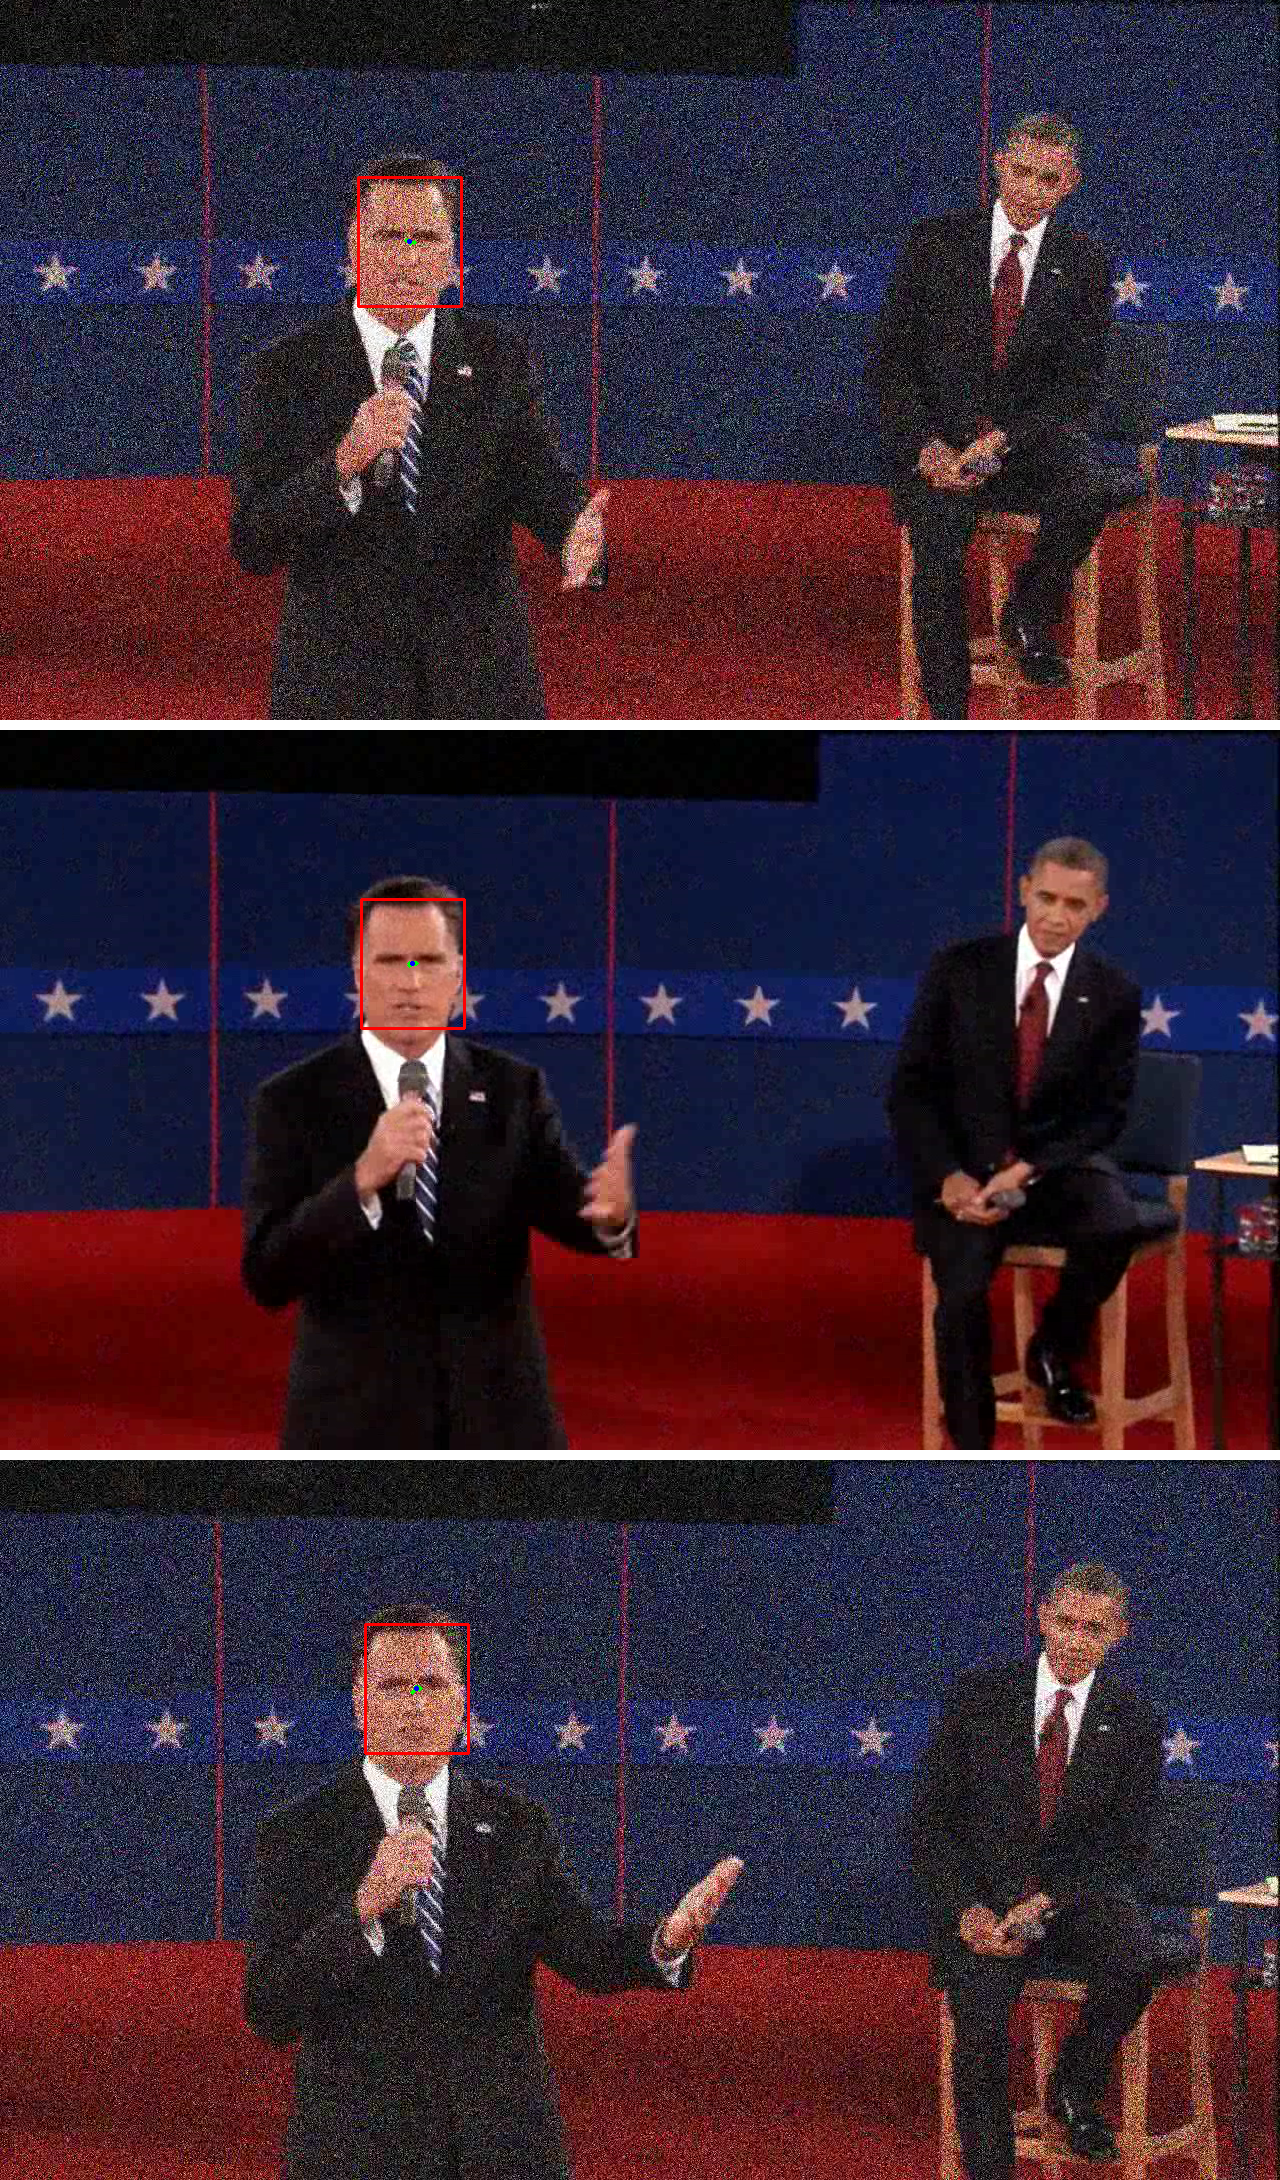
\includegraphics[height=1 \textwidth]{ps6-1-5-frames1-14-32-46.png}\\
\end{tabular}
\end{center}
\caption{ps6-1-5-frames1-14-32-46.png}
\label{ps-6-5-a}
\end{figure}

\begin{figure}[H]
\begin{center}
\begin{tabular}{c}
	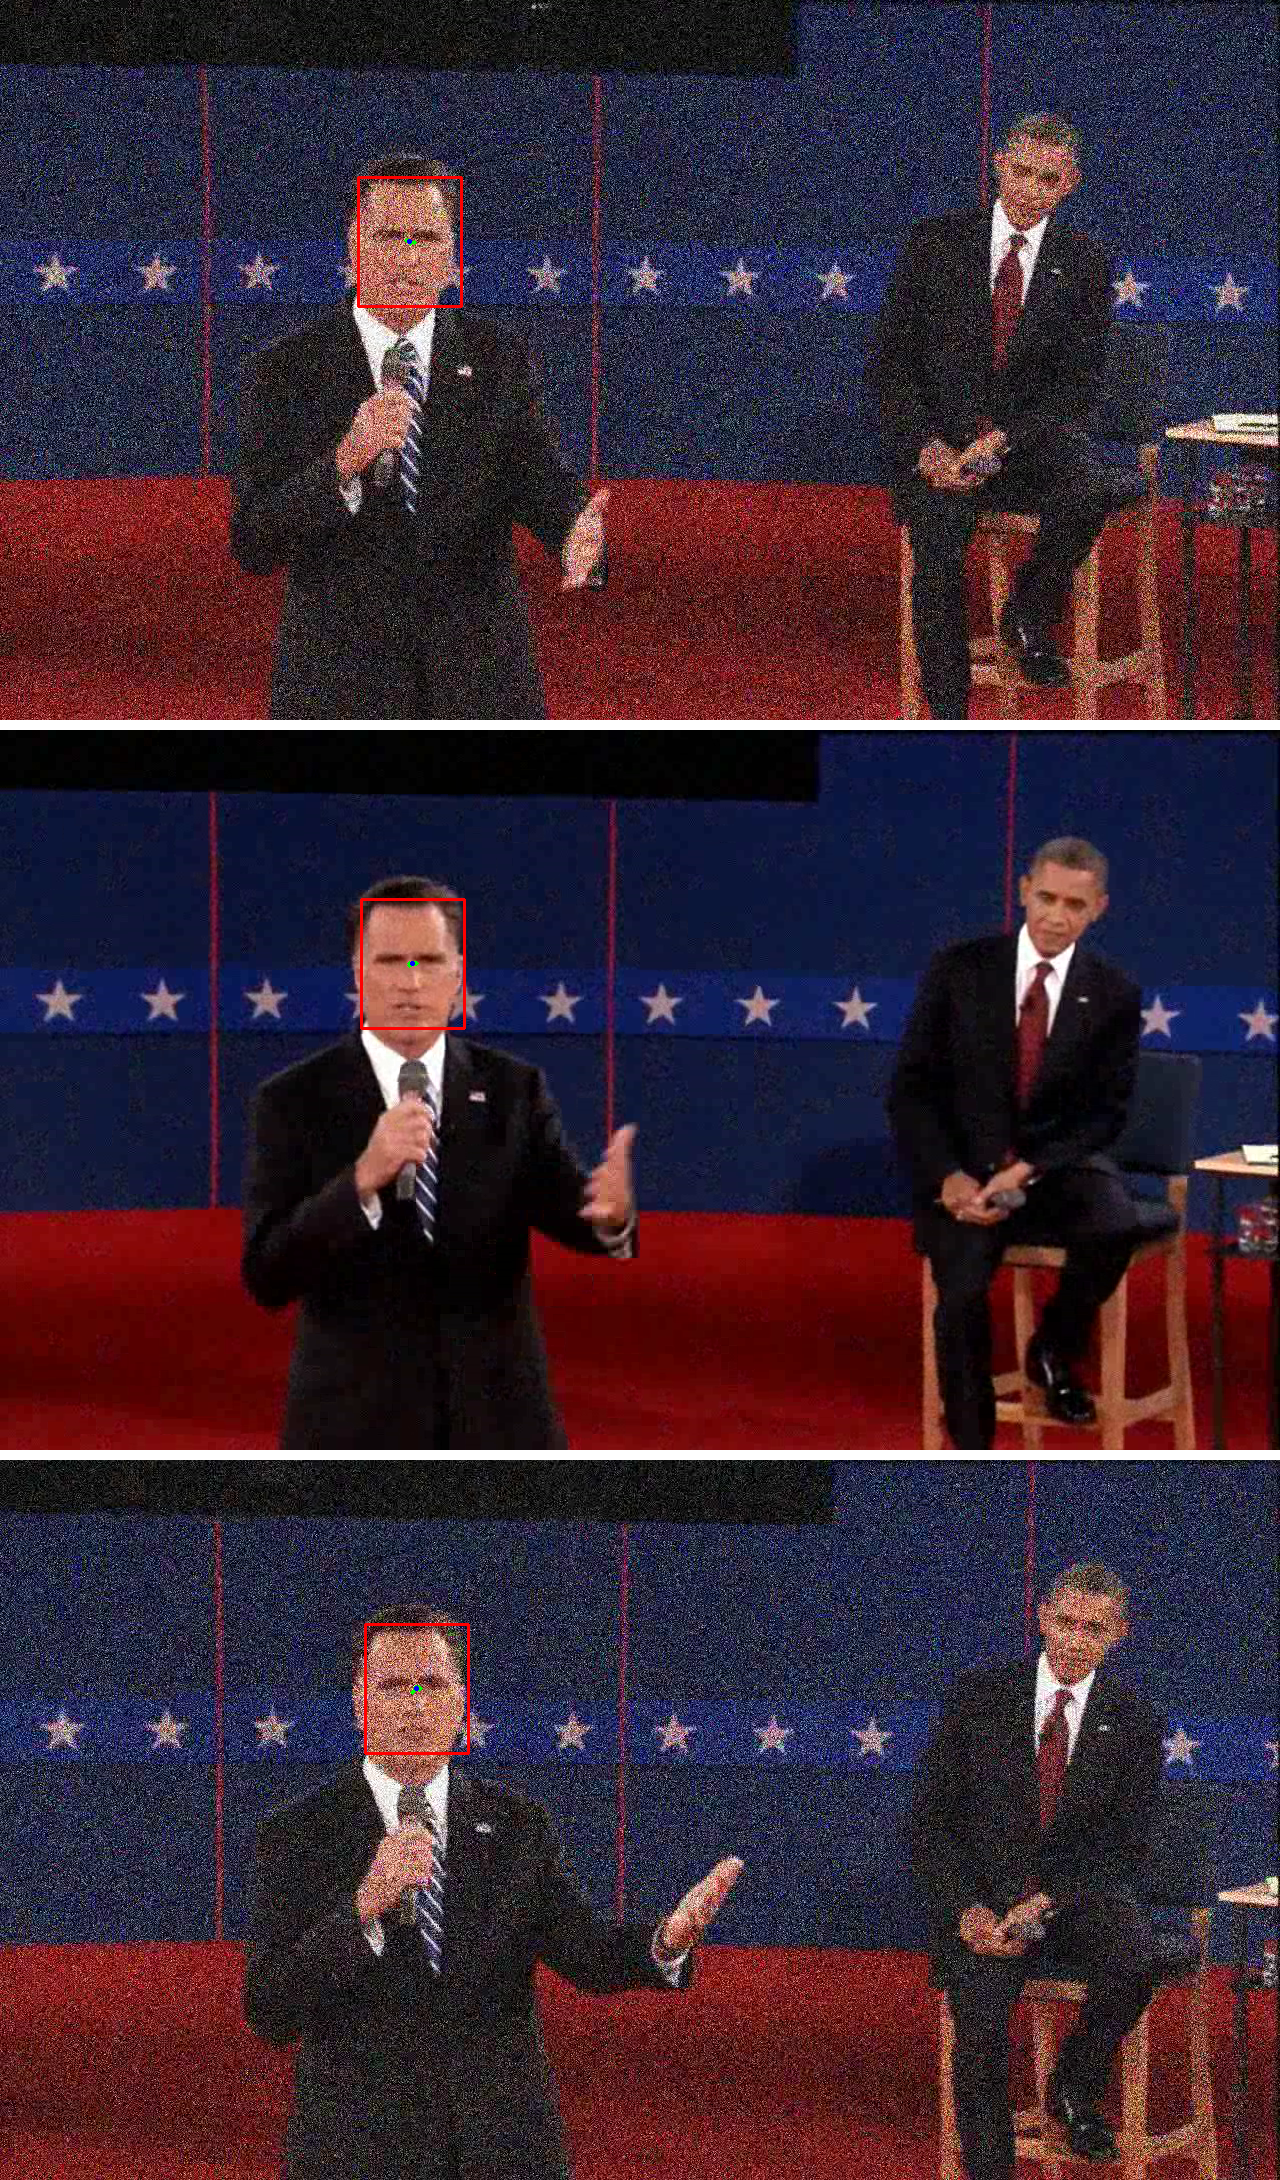
\includegraphics[height=1 \textwidth]{ps6-1-5-frames1-14-32-46.png}\\
\end{tabular}
\end{center}
\caption{ps6-1-5-frames1-14-32-46.png}
\label{ps-6-5-b}
\end{figure}

The three trackers do fairly well at tracking Romney's face, and all three offer the same response to an increasing level of noise. In this situation, the particles all tend to spread out around the mean value.
The large value of $\sigma_{MSE}$ (Figure 11), as explained above, gives a result that is not very smooth and particles get spread in noisy phases. The middle value gives a cleaner tracking but for this particular case we would probably choose the lowest (Figure 10) of the 3, because it is less sensitive to the varying noise (particles spread less easily).
If the noise bursts were longer, a small $\sigma_{MSE}$ would probably help in keeping a good track of Romney's face, while higher values would see their mean keep increasing.


\section{Appearance Model Update}

\subsection{Appearance Model Update}

We now wish to track the hand of Romney, which is see at different angles throughout the video. We thus need to update the template in order to make it evolve with the movement. This is done in the new function shown below.\\

We also decide to take a small initial template, which does not cover the full hand (Figure 13). This helps in focusing on the hand and discarding as much of the background as possible.

\begin{table}[H]
\centering
\caption{Parameters}
%\label{my-label}
\begin{tabular}{|l|l|}
\hline
    MSE standard deviation   &   10.0 \\ \hline
    Initial noise standard deviation &  [ 5.  5.  0.] \\ \hline
    Predict noise standard deviation &  [ 20.  20.  0.] \\ \hline
    Number of particles &  100 \\ \hline
    Alpha   & 0.2\\ \hline
\end{tabular}
\end{table}

\begin{figure}[H]
\begin{center}
\begin{tabular}{c}
	\includegraphics[height=1 \textwidth]{ps6-2-1-frames-15-50-140.png}\\
\end{tabular}
\end{center}
\caption{ps6-2-1-frames-15-50-140.png}
\label{ps-6-6-a}
\end{figure}

\begin{figure}[H]
\begin{center}
\begin{tabular}{c}
	\includegraphics[height=.2 \textwidth]{ps6-2-1-template.png}\\
\end{tabular}
\end{center}
\caption{ps6-2-1-template.png}
\label{ps-6-5-b}
\end{figure}

Moreover, we increase the standard deviation on the dynamics model and the number of particles so that we get a better chance at having some particles to follow the hand, especially since it moves much faster than the head.\\
Finally, the constant value $\alpha$ used in the template update step is chosen to be low, so that changes in appearance is taking into account slowly (history has more weight). Indeed since our template is limited to a small portion of the hand, we suppose it won?t change too fast in appearance.\\
The result is visible in Figure 12.

\lstset{style=mystyle}
\lstinputlisting[language=Python, firstline=91, lastline=105]{/Users/melisandezonta/Documents/Documents/Documents/GTL_courses_second_semester/Computer-Vision/PS6-all/PS6-code/Functions.py}

\subsection{Noisy Tracking on Romney's Hand}

The same template is now tracked in the noisy version of the debate.

\begin{table}[H]
\centering
\caption{Parameters}
%\label{my-label}
\begin{tabular}{|l|l|}
\hline
    MSE standard deviation   &   10.0 \\ \hline
    Initial noise standard deviation &  [ 5.  5.  0.] \\ \hline
    Predict noise standard deviation &  [ 20.  20.  0.] \\ \hline
    Number of particles &  200 \\ \hline
    Alpha   & 0.01\\ \hline
\end{tabular}
\end{table}

\begin{figure}[H]
\begin{center}
\begin{tabular}{c}
	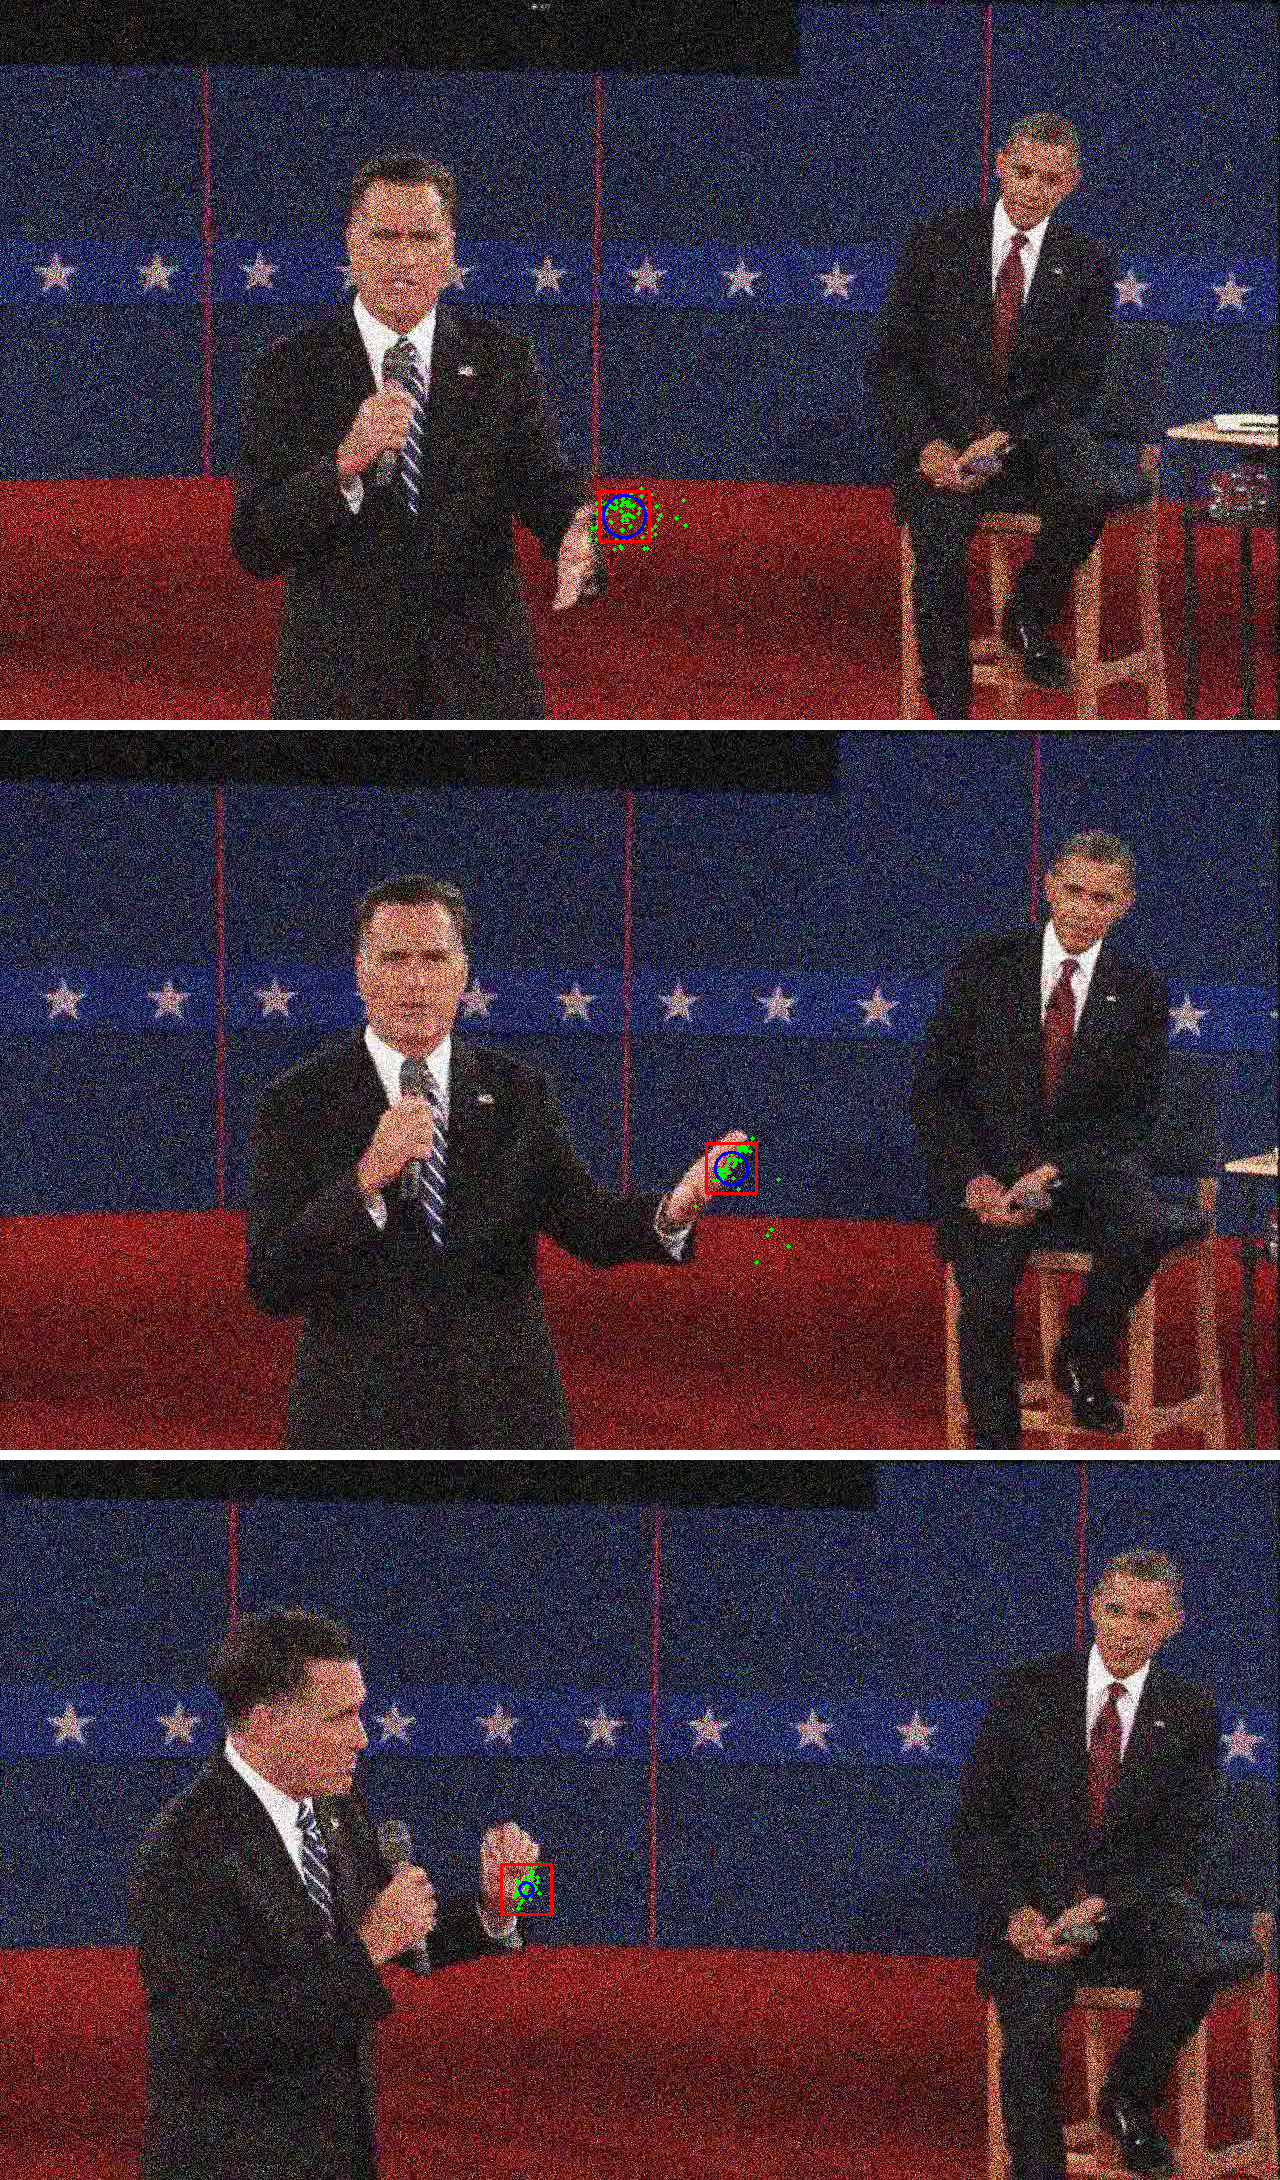
\includegraphics[height=1 \textwidth] {ps6-2-2-frames-15-50-140.png}\\
\end{tabular}
\end{center}
\caption{ps6-2-2-frames-15-50-140.png}
\label{ps-6-5-b}
\end{figure}
    
We decide to increase the number of particles and reduce the value of $\alpha$ in order to be more robust to the noise.\\
Reducing alpha especially appears to be very important, since it gives a very large weight to the history in order to limit the impact of the noise on the template update.\\
Although on the first frames it appears that the mean of the tracker gets further away from the hand, some particles drag it back and we do not loose it in the long run.\\
We manage to get good results (Figure 14) but they are not necessarily consistent over several tests. However, we decide to keep it as such and limit the number of modified parameters in order to be able to compare the results with the normal version of the video.



\section{Incorporating More Dynamics}

\subsection{Pedestrian Tracking}


The next challenge is to deal with occlusion on a new video with pedestrians crossing the road, thus getting further away from the fixed camera.\\
We first need to adapt the template scale along the course of the video in order to account for the increasing distance to the target, which is done in the code below.\\
However, we no longer update the template according to the history, since the target orientation does not change in the first part of the video. This makes the content of the initial template (Figure 16) still relevant after many frames.\\

\begin{table}[H]
\centering
\caption{Parameters}
%\label{my-label}
\begin{tabular}{|l|l|}
\hline
    MSE standard deviation   &   10.0 \\ \hline
    Initial noise standard deviation &  [ 0.1  0.1  0.1] \\ \hline
    Predict noise standard deviation &  [ 0.5  0.5  0.2] \\ \hline
    Number of particles &  200 \\ \hline
\end{tabular}
\end{table}

We keep the default value for $\sigma_{MSE}$ but force much lower values on the standard deviation for the x and y coordinates, since the position of the center does not move very much in the first hundred frames (only the scale). The standard deviation for the scale is then set to a reasonably high level, so that when scale tends to get lost during the occlusion it can be recovered efficiently afterwards.\\
The result is visible in Figure 15.

\begin{figure}[H]
\begin{center}
\begin{tabular}{c}
	\includegraphics[height=1 \textwidth] {ps6-3-1-frames-40-100-240.png}\\
\end{tabular}
\end{center}
\caption{ps6-3-1-frames-40-100-240.png}
\label{ps-6-5-b}
\end{figure}


\begin{figure}[H]
\begin{center}
\begin{tabular}{c}
	\includegraphics[height=.2 \textwidth] {ps6-3-1-template.png}\\
\end{tabular}
\end{center}
\caption{ps6-3-1-template.png}
\label{ps-6-5-b}
\end{figure}

\subsection{Pedestrian Tracking Optimization}

The last step, once more, is to find an optimal number of particles to track the pedestrian.

\begin{table}[H]
\centering
\caption{Parameters}
%\label{my-label}
\begin{tabular}{|l|l|}
\hline
    MSE standard deviation   &   10.0 \\ \hline
    Initial noise standard deviation &  [ 0.1  0.1  0.1] \\ \hline
    Predict noise standard deviation &  [ 0.5  0.5  0.2] \\ \hline
    Number of particles &  100 \\ \hline
\end{tabular}
\end{table}

Here again, we try to reduce the number of particles while keeping a relatively "stable" tracking. We settle on 100 particles, with a result visible in Figure 17. The scale parameter is still very unstable during the occlusion, but it gets back quickly on target while not "shaking" too much. Below this, we also increase the risk that the scale parameter is not properly recovered after the occlusions.
This number is more than 3 times higher than what we found in question 1.4.

\begin{figure}[H]
\begin{center}
\begin{tabular}{c}
	\includegraphics[height=1 \textwidth] {ps6-3-2-frames-40-100-240.png}\\
\end{tabular}
\end{center}
\caption{ps6-3-2-frames-40-100-240.png}
\label{ps-6-5-b}
\end{figure}


\begin{table}[thpb]
\centering
\caption{Tasks Planning}
\label{my-label}
\begin{tabular}{|l|l|l|l|l|}
\hline
 & Setting up environment & \begin{tabular}[c]{@{}l@{}}Data processing \& \\ augmentation pipeline\end{tabular} & \begin{tabular}[c]{@{}l@{}}Net architecture,\\  train, test\end{tabular} & Results analysis \\ \hline
Badr & X &  &  X&  \\ \hline
Melisande &  &  &  X&  \\ \hline
Mohammed &  &  &  X&  \\ \hline
Vincent &  & X & X & X \\ \hline
 & \begin{tabular}[c]{@{}l@{}}Write-up intro \&\\ contextualization\end{tabular} & \begin{tabular}[c]{@{}l@{}}Write-up \\ Technical details\end{tabular} & Poster & Report Formatting \\ \hline
Badr & X &  &  &  \\ \hline
Melisande &  & X & X & X \\ \hline
Mohammed &  & X & X & X  \\ \hline
Vincent &  &  &  &  \\ \hline
\end{tabular}
\end{table}


\end{document}